\section{Evaluering}

\subsection{H�jttaleren isoleret set}

Med NXT'en f�lger en r�kke lydfiler med tale. Frekvensen af forst�elig tale ligger mellem 300 og 3000 Hz, og filerne er i 8 kHz, s� NXT'ens h�jttaler vil fint kunne frembringe dette. 'Bip-lyde' med et begr�nset frekvensspektrum vil liges� kunne afspilles, mens frembringelse af musik, hvor frekvensspektret er noget bredere, er mere problematisk. Specielt frekvensdykket omkring 2 kHz p� ca. 10 dB vil p�virke musikken i n�vnev�rdig grad.

Der vil dog v�re problemer med dybe frekvenser op til 600 Hz, s� f.eks. mandetale vil lyde tynd. En bedre gengivelse af tale i dybe frekvenser ville kr�ve st�rre driver, hvilket kan have p�virket LEGOs valg.

\subsection{Lydkredsl�b sammenholdt med h�jttaler}
Peter V�dele Clausen har i sit speciale\footnote{Se \texttt{http://www.daimi.au.dk/\~{}u991789/}} analyseret den del af NXT'ens lydkredsl�b, der kommer f�r h�jttaleren. Iflg. ham har NXT'en ikke en egentlig A/D-converter, men benytter sig af Pulse Width Modulation (PWM) til at frembringe lyden. Konverteringen fra PCM til PWM bevirker at der genereres en m�ngde h�jfrekvens st�j, hvilket i NXT'en fjernes med et lavpas-filter. Peter V�dele Clausen har vha. et sinus-sweep m�lt frekvensresponset p� kredsl�bet samt det analoge filter, vist i figur \ref{circuit}.

% kredsl�b og filter
\begin{figure}
\begin{center}
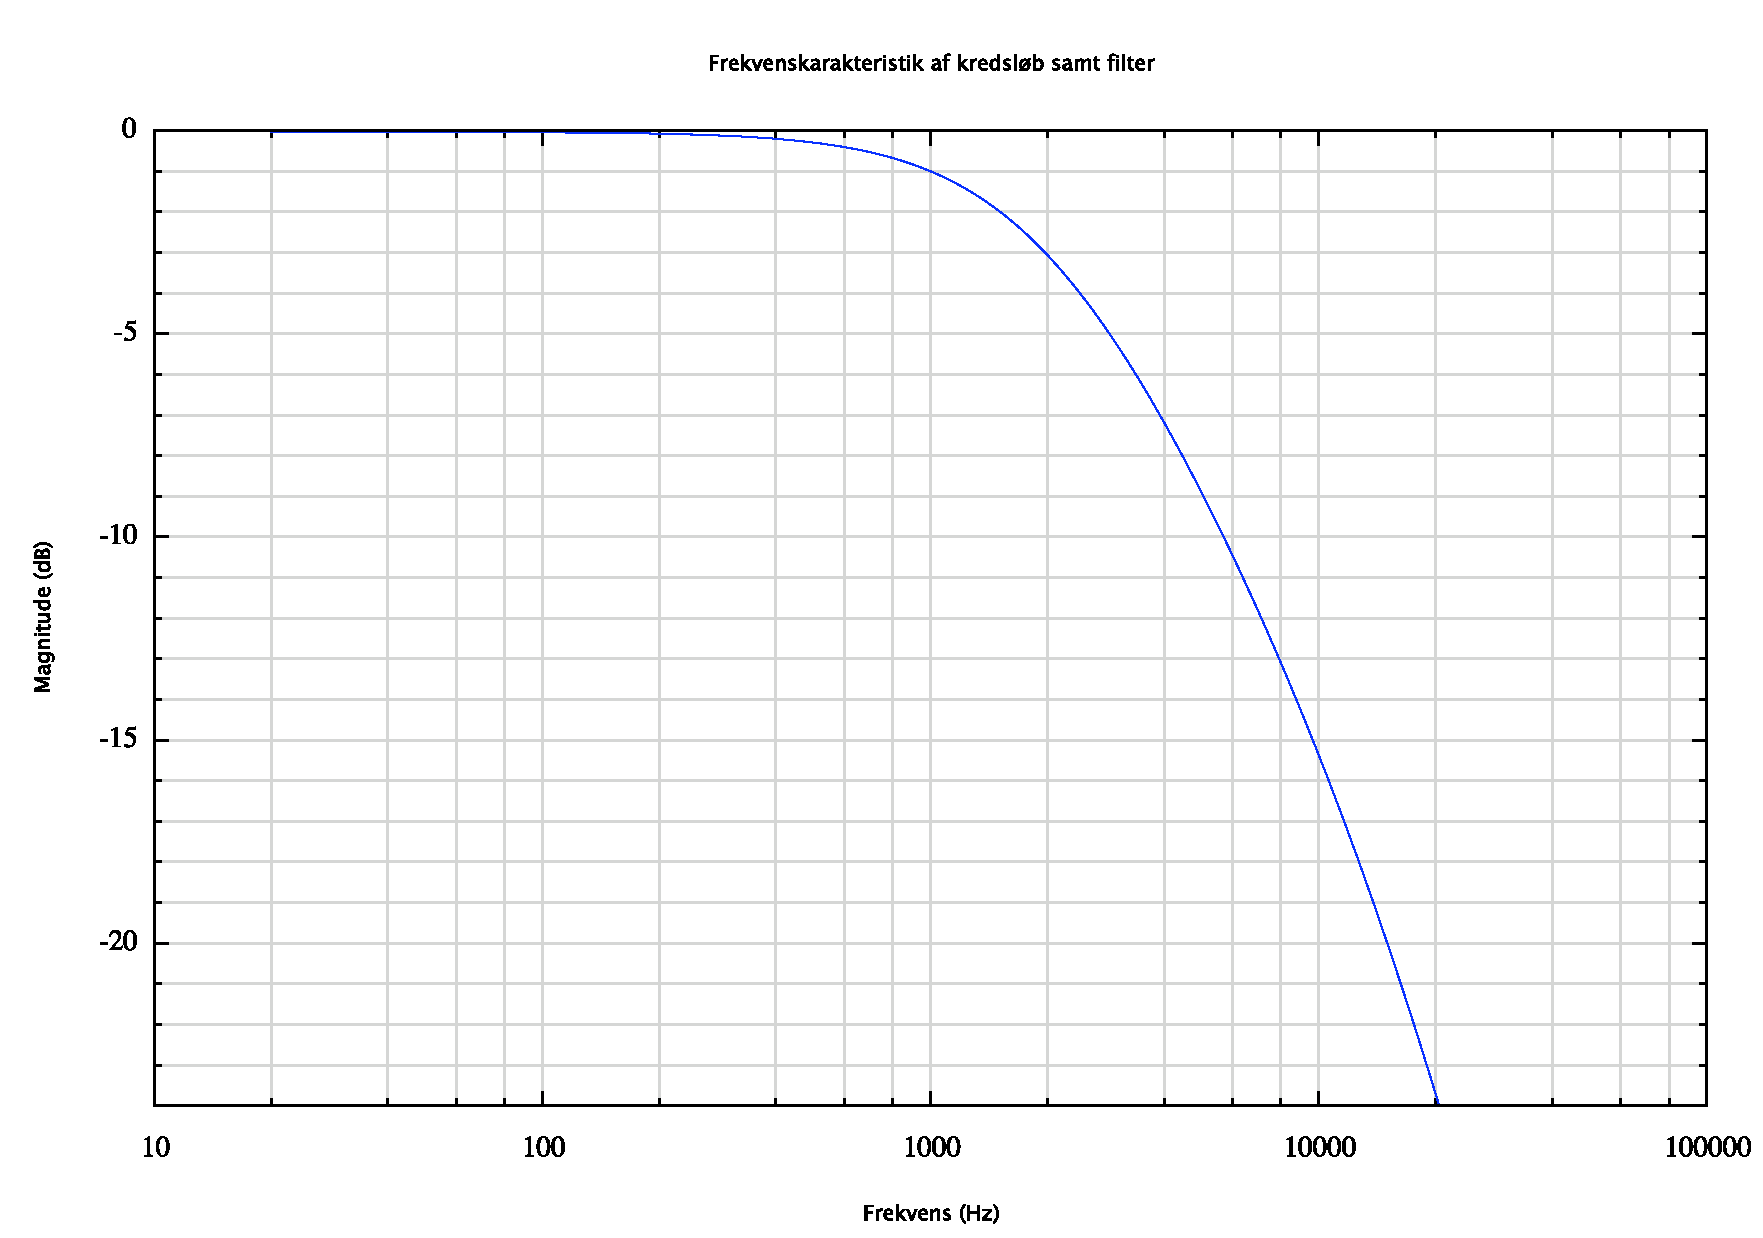
\includegraphics[width=12cm]{circuit-filter.pdf}
\end{center}
\caption{Digitalt kredsl�b samt analogt filter i NXT}
\label{circuit}
\end{figure}

%

Som det fremg�r af figur \ref{circuit}, bevirker NXT'ens kredsl�b sammen med det analoge filter et fald p� 3 dB ved omkring 2 kHz, mens h�jttaleren f�rst begynder at respondere ved 600 Hz. Som det fremg�r af figur \ref{onaxis}, har h�jttaleren med kabinet endvidere et dyk omkring de 2 kHz. 

Dette g�r det samlede system i stand til nogenlunde line�rt at frembringe frekvenser fra ca. 600 til 2000 Hz, hvilket er et meget sn�vert frekvensb�nd, s� her diskvalificeres systemet fuldst�ndigt til at spille musik, mens tale og 'bip-lyde' stadig kan frembringes med nogenlunde kvalitet, dog med en vis negativ p�virkning af forst�eligheden af talen.

\subsection{Korrektion}
En digital korrektion vil kunne oprette dykket omkring 2 kHz, men den vil ikke kunne forbedre den smalle frekvensrespons, hvilket er det samlede systems st�rste problem. Dermed vil en digital korrektion i sidste ende ikke g�re den store forskel.


 